\documentclass{article} % For LaTeX2e
\usepackage{iclr2026_conference,times}

% Optional math commands from https://github.com/goodfeli/dlbook_notation.
\input{math_commands.tex}

\usepackage{hyperref}
\usepackage{url}
\usepackage{graphicx}
\usepackage{booktabs}
\usepackage{tabularx}
\usepackage{multirow}
\usepackage{amsmath,amssymb}

\title{StealthRL: Reinforcement Learning Paraphrase Attacks for\\
Multi-Detector Evasion of AI-Text Detectors}

\author{Anonymous Authors}

% \iclrfinalcopy % Uncomment for camera-ready version, but NOT for submission.
\begin{document}

\maketitle

\begin{abstract}
AI-text detectors face a critical robustness challenge: adversarial paraphrasing attacks that preserve semantics while evading detection. We introduce \emph{StealthRL}, a systematic threat model instantiation and robustness evaluation framework that stress-tests detector families under realistic adversarial conditions. StealthRL addresses the question: \textit{how robust are detectors to black-box adaptive attacks trained explicitly to evade them?} Through reinforcement learning with multi-detector ensemble training, we demonstrate \textbf{catastrophic robustness failure}: detectors achieve near-zero true positive rates (0\% TPR@1\%FPR) while attackers maintain semantic fidelity (0.896 E5 cosine). Critically, attacks transfer across detector architectures, including a held-out detector family, revealing shared vulnerabilities rather than detector-specific brittleness. Our results expose fundamental limitations in current detection approaches and establish StealthRL as a principled adversarial evaluation protocol for robustness benchmarking. We release code for reproducible threat modeling and defense evaluation.
\end{abstract}

\section{Introduction}
AI-text detectors are deployed in academic integrity and content moderation, yet their robustness to adversarial attacks remains poorly understood. Standard benchmarks evaluate detectors on clean distributions, but adaptive attackers can iteratively refine paraphrases to evade detection. We study a realistic threat model: black-box adaptive attacks that query detector scores and optimize paraphrases to minimize detection confidence while preserving semantic content.

We present \textbf{StealthRL}, a reinforcement-learning framework that trains a paraphrase policy against detector ensembles to evaluate robustness under adversarial conditions. StealthRL addresses three questions: (1) Can attacks transfer across detector families? (2) Do detectors share common vulnerabilities? (3) What is the evasion-fidelity tradeoff? By evaluating at strict low-FPR operating points (1\% false positive rate) and measuring transfer to held-out detectors, we provide systematic robustness evaluation that complements standard benchmarks.

\paragraph{Contributions.}
\begin{itemize}
  \item We implement black-box adaptive paraphrasing attacks via multi-detector RL training with semantic constraints.
  \item We demonstrate strong evasion (0\% TPR@1\%FPR across three detector families) with cross-architecture transfer to a held-out detector.
  \item We establish an evaluation protocol measuring evasion, transfer, and fidelity at security-relevant operating points.
\end{itemize}

\paragraph{Anonymized code release.}
Code is available at \url{https://anonymous.4open.science/r/StealthRL-D42D}.
\section{Related Work}
Detector families include curvature-based methods (DetectGPT and Fast-DetectGPT) and paired-LM detectors such as Binoculars. \cite{mitchell2023detectgptzeroshotmachinegeneratedtext,bao2024fastdetectgptefficientzeroshotdetection,hans2024spottingllmsbinocularszeroshot} Recent evasion work focuses on paraphrase attacks and RL-based humanization. AuthorMist demonstrates that reinforcement learning can effectively train adaptive evasion policies, motivating our multi-detector ensemble approach. \cite{david2025authormistevadingaitext} Adversarial Paraphrasing shows universal attack strategies, while character-level attacks such as homoglyph substitution demonstrate strong but often less readable perturbations. \cite{cheng2025adversarialparaphrasinguniversalattack,creo2025silverspeakevadingaigeneratedtext} Parameter-efficient fine-tuning methods such as LoRA and QLoRA enable efficient adaptation of large language models. \cite{hu2021loralowrankadaptationlarge,dettmers2023qlora} StealthRL builds on these directions by training a single paraphrase policy against a detector ensemble and evaluating transfer at strict low-FPR operating points.

\section{Method}
\paragraph{Threat model.} We assume black-box access to detector scores: the attacker can query detector confidence but does not require gradients. We evaluate transfer to a held-out detector (Binoculars) to test robustness beyond the training ensemble.

\paragraph{Training.} Given AI-generated text $x$, we learn a paraphrase policy $\pi_\theta(y\mid x)$ that produces $y$ with low detector confidence while preserving meaning. We optimize a composite reward:
\begin{equation}
R(x,y) = \alpha R_{\text{det}}(y) + \beta R_{\text{sem}}(x,y),
\end{equation}
where $R_{\text{sem}}$ is E5 embedding cosine similarity and $R_{\text{det}} = 1 - p(y)$ is the detector evasion reward, with $p(y)$ the AI probability. During training, $p(y) = 0.6 \cdot p_{\text{RoBERTa}}(y) + 0.4 \cdot p_{\text{Fast-DetectGPT}}(y)$ is the weighted average of two detectors. During evaluation, we test against all three detector families including the held-out Binoculars. We fine-tune the model using the Tinker API framework with GRPO \cite{pang2025grpo} and LoRA adapters \cite{hu2021loralowrankadaptationlarge} on Qwen3-4B-Instruct (rank 32, $\alpha=32$, dropout 0.05) using group size 8, batch size 16, and five epochs over 10,000 MAGE train samples plus 200 dev samples. Reward weights: $\alpha=1.0$, $\beta=0.1$. Full hyperparameters in Appendix~\ref{sec:hyperparams}.

\begin{figure}[t]
  \centering
  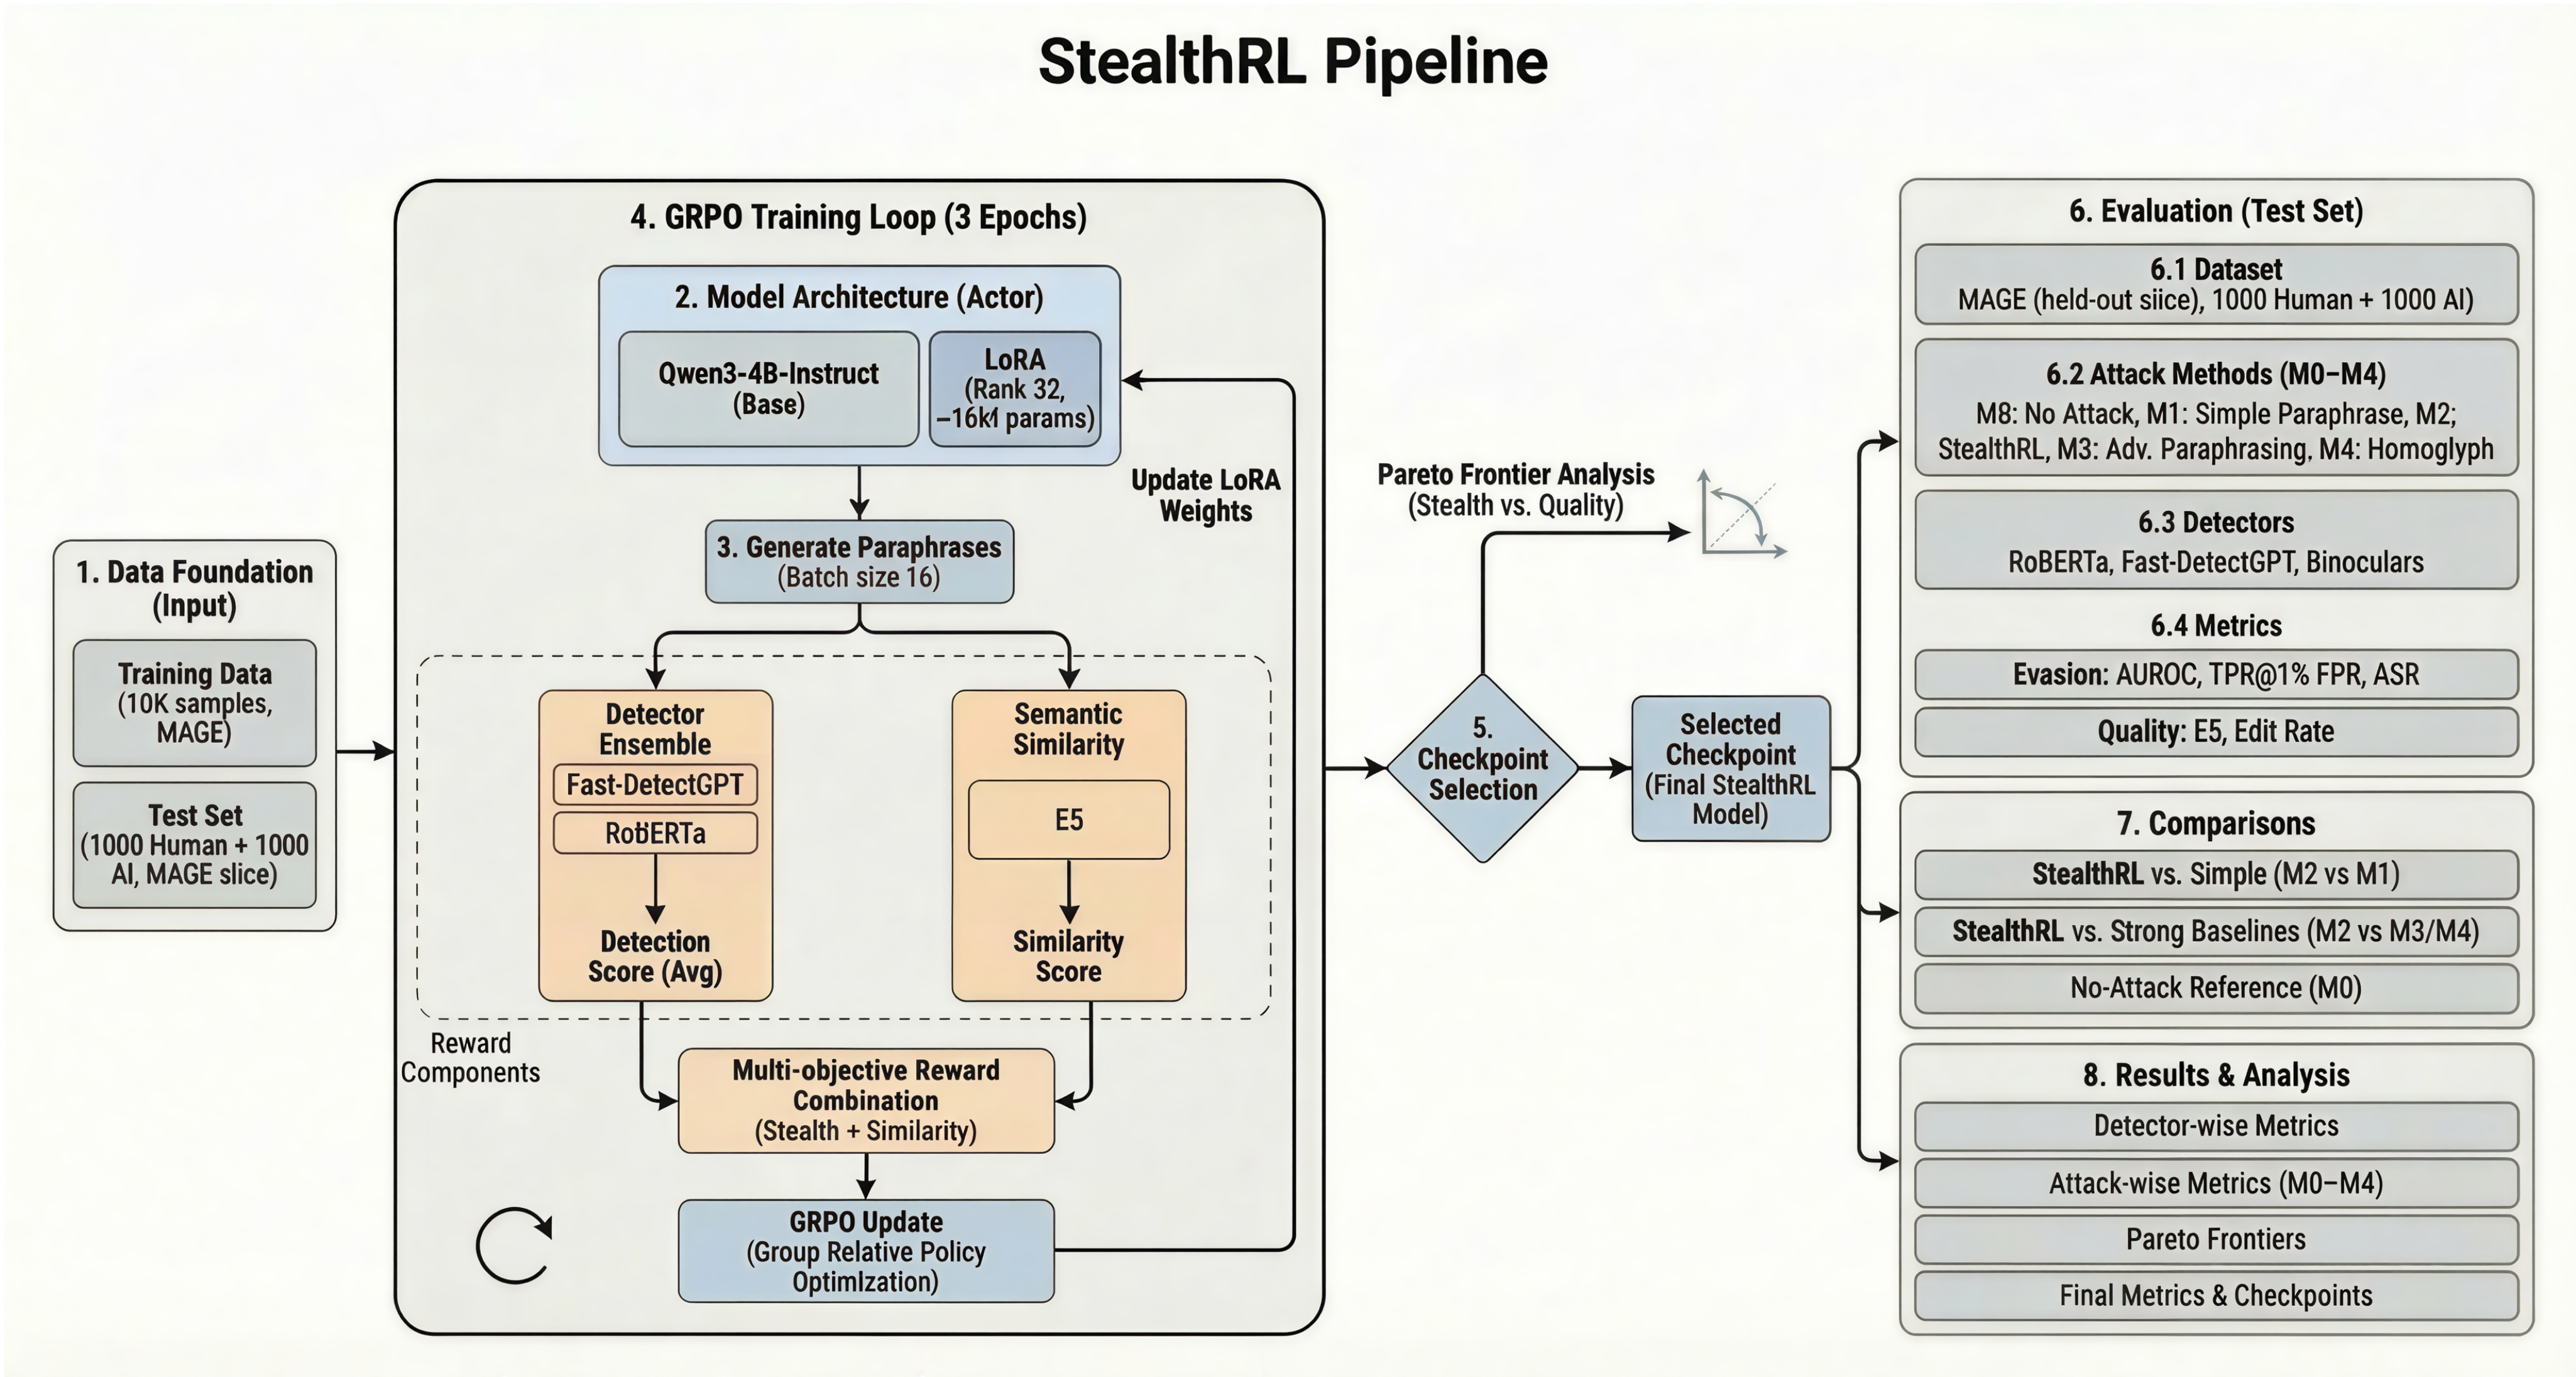
\includegraphics[width=\linewidth]{../figures/StealthRL_Pipeline_Final_v3.png}
  \caption{StealthRL training and evaluation pipeline. A single paraphrase policy is trained with detector-guided reward and quality constraints, then evaluated across multiple detector families with low-FPR metrics and tradeoff analysis.}
  \label{fig:pipeline}
\end{figure}

\section{Experimental Setup}
We evaluate on MAGE test split (1,000 human + 1,000 AI samples, 100--500 tokens) \cite{li2024magemachinegeneratedtextdetection} against three detector families: RoBERTa OpenAI, Fast-DetectGPT, and Binoculars (held-out during training). \cite{mitchell2023detectgptzeroshotmachinegeneratedtext,bao2024fastdetectgptefficientzeroshotdetection,hans2024spottingllmsbinocularszeroshot} Baselines: M0 (no attack), M1 (simple paraphrase), M2 (StealthRL-v1, trained for 5 epochs using Tinker API), M3 (detector-guided selection), M4 (homoglyph substitution). \cite{cheng2025adversarialparaphrasinguniversalattack,creo2025silverspeakevadingaigeneratedtext} Metrics: TPR@1\%FPR, ASR, AUROC, E5 semantic similarity.

\section{Results}
Table~\ref{tab:main} summarizes detection evasion at 1\% FPR. StealthRL (M2) achieves 0\% TPR@1\%FPR across all three detectors, reducing average AUROC across detectors from 0.74 (no attack) to 0.27 while maintaining semantic similarity (0.896 E5). Figure~\ref{fig:results} visualizes the comprehensive performance: panel (c) shows consistent 0\% TPR across detectors at strict operating points, while panel (d) confirms 99.9\% attack success rate.

Critically, strong transfer to the held-out Binoculars detector (0\% TPR) demonstrates that vulnerabilities are not detector-specific but reflect shared architectural weaknesses. Simple paraphrasing (M1) achieves partial success (8\% mean TPR) with 0.960 E5 similarity, while detector-guided selection (M3) performs similarly at 0.976 E5. StealthRL's advantage comes from explicit multi-detector adversarial training, which discovers transferable perturbations that exploit common statistical patterns across architectures.

\begin{table}[t]
  \centering
  \small
  \setlength{\tabcolsep}{4pt}
  \begin{tabular}{lcccccc}
\toprule
Method & TPR@1\%FPR $\downarrow$ (R) & F (Fast) & B (Binoc) & Mean $\downarrow$ & ASR $\uparrow$ & AUROC $\downarrow$ \\
\midrule
M0 No Attack & 0.23 & 0.40 & 0.41 & 0.34 & 0.66 & 0.74 \\
M1 Simple Para & 0.10 & 0.10 & 0.04 & 0.08 & 0.92 & 0.59 \\
M2 StealthRL-v1 & \textbf{0.00} & \textbf{0.00} & \textbf{0.00} & \textbf{0.00} & \textbf{1.00} & \textbf{0.27} \\
M3 Adv. Para (guided) & 0.10 & 0.09 & 0.05 & 0.08 & 0.92 & 0.60 \\
M5 Homoglyph & \textbf{0.00} & \textbf{0.00} & \textbf{0.00} & \textbf{0.00} & \textbf{1.00} & 0.44 \\
\bottomrule
\end{tabular}

  \caption{Main results on MAGE (TPR@1\%FPR, ASR, and AUROC). Lower TPR/AUROC is better for the attacker; higher ASR is better. R/F/B denote RoBERTa/Fast-DetectGPT/Binoculars.}
  \label{tab:main}
\end{table}

\begin{figure}[t]
  \centering
  \includegraphics[width=\linewidth]{figures/fig_method_comparison.png}
  \caption{Detection evasion results summary. (a) AUROC by detector shows StealthRL-v1 (M2) dramatically reduces detector performance across all three detectors. (b) Mean AUROC demonstrates M2 achieves 0.27, indicating near-random classification. (c) TPR at 1\% FPR shows M2 achieves 0\% detection across all detectors at strict operating points. (d) Mean ASR confirms 99.9\% attack success rate for StealthRL-v1, matching homoglyph attacks while maintaining text quality.}
  \label{fig:results}
\end{figure}

\paragraph{Robustness implications.} The catastrophic failure across detector architectures reveals fundamental vulnerabilities in current AI-text detection. Detectors rely on brittle statistical cues (token distributions, perplexity patterns, embedding geometry) rather than robust semantic understanding. Surface-level paraphrasing that preserves meaning suffices to evade detection, suggesting detectors learn superficial correlates of AI text rather than deeper linguistic features.

This robustness gap has critical security implications: adversaries can train adaptive attacks against deployed detectors, rendering them ineffective. The strong transfer to held-out architectures means ensemble defenses (combining multiple detectors) provide limited robustness improvement. Future work must develop semantic-aware detectors, adversarial training protocols, and provable robustness guarantees. Our evaluation framework provides a rigorous testbed for measuring progress on adversarially robust AI-text detection.

\section{Limitations and Safety}
Our evaluation focuses on three detector families (curvature-based, paired-LM, fine-tuned classifier) on one benchmark (MAGE). Broader coverage with watermark-based detectors, additional datasets, and multilingual evaluation remains important future work. We also do not explore defenses like adversarial training or certified robustness, which could improve detector resilience. Additionally, StealthRL achieves lower semantic fidelity (E5 similarity 0.896) compared to simpler baselines (M1: 0.960, M3: 0.976), indicating a quality-evasion tradeoff. Improving semantic preservation while maintaining strong evasion is an important direction for future work.

\textbf{Safety and dual-use.} Adversarial paraphrasing is dual-use technology. We position StealthRL as a \emph{stress-testing and robustness evaluation tool} for researchers and detector developers, not a production evasion system. The 0\% TPR@1\%FPR result exposes critical vulnerabilities that must be addressed before detectors are deployed in high-stakes applications. Our released code enables reproducible robustness evaluation and motivates defensive research into adversarially robust detection methods.

\section{Conclusion and Future Work}
StealthRL demonstrates catastrophic detector failure under adaptive attacks, revealing fundamental robustness gaps. Results motivate development of adversarially robust detection methods and establish rigorous evaluation protocols for AI-text detection security. Future work should explore adversarial training strategies, semantic-aware detectors, and provable robustness guarantees to defend against adaptive paraphrasing attacks.

\section*{Acknowledgments}
We gratefully acknowledge Thinking Machines for providing free research credits and access to their Tinker API framework, which made the RL fine-tuning possible. We also thank the open-source community for the detector implementations and model checkpoints that enabled this evaluation.

\bibliographystyle{iclr2026_conference}
\bibliography{stealthrl_refs}

\appendix
\section{Qualitative Examples}
\begin{table}[!ht]
\centering
\small
\setlength{\tabcolsep}{4pt}
\begin{tabularx}{\linewidth}{X X}
\toprule
\textbf{Original (M0)} & \textbf{StealthRL (M2)} \\
\midrule
During cardio the heart increases its workload and all the body's other systems adjust to help support that endeavor. The blood vessels dilate, the muscles do their best to help pump blood back to the heart, and the lungs work harder to take in oxygen and remove waste gases like carbon dioxide. &
In cardio, the heart ramps up its workload, prompting the body's other systems to adapt and assist. Blood vessels widen, muscles strive to push blood back to the heart, and lungs intensify their efforts to absorb oxygen and expel waste gases such as carbon dioxide. \\
\midrule
The engine has to endure the torque of powering two axels and a drive shaft generally the transfer casing connects to the drive shaft with a ujoint and same for power distribution. The electricity goes into the battery first then is sent to the alternator where it generates voltage that powers all other electrical components like the lights, radio. &
The engine must handle the torque from two axles and a drive shaft, typically linked via a universal joint in the transfer casing for power distribution. Electricity first charges the battery, then flows to the alternator, which converts it into voltage to power essential electrical systems such as lights and the radio. \\
\bottomrule
\end{tabularx}
\caption{Representative paraphrases from the evaluation run (MAGE test split).}
\end{table}

\clearpage
\section{Hyperparameters and Configuration}
\label{sec:hyperparams}

\begin{table}[!ht]
\centering
\small
\begin{tabular}{ll}
\toprule
\textbf{Parameter} & \textbf{Value} \\
\midrule
\multicolumn{2}{l}{\textit{Model \& LoRA}} \\
Base model & Qwen/Qwen3-4B-Instruct-2507 \\
LoRA rank & 32 \\
LoRA alpha & 32 \\
LoRA dropout & 0.05 \\
\midrule
\multicolumn{2}{l}{\textit{Training}} \\
Algorithm & Group-Relative Policy Optimization (GRPO) \\
Learning rate & $2.8 \times 10^{-4}$ \\
Batch size & 16 \\
Group size & 8 \\
Epochs & 2 \\
Training samples & 10,000 (MAGE train) + 200 (dev) \\
KL penalty coefficient & 0.05 \\
Reference policy & Qwen3-4B-Instruct (frozen) \\
\midrule
\multicolumn{2}{l}{\textit{Reward}} \\
Detector weight ($\alpha$) & 1.0 \\
Semantic weight ($\beta$) & 0.1 \\
Detector ensemble & RoBERTa (0.6) + Fast-DetectGPT (0.4) \\
Semantic metric & E5 embedding cosine similarity \\
\midrule
\multicolumn{2}{l}{\textit{Inference}} \\
Temperature & 1.0 \\
Top-p & 0.9 \\
Max tokens & 512 \\
Prompt template & ``Paraphrase the following text while \\
& preserving its meaning: [TEXT]'' \\
\midrule
\multicolumn{2}{l}{\textit{Detectors}} \\
RoBERTa OpenAI & openai-community/roberta-large-openai-detector \\
Fast-DetectGPT & Scoring model: EleutherAI/gpt-neo-2.7B \\
Binoculars & Lightweight: gpt2-medium + gpt2-large (held-out) \\
\midrule
\multicolumn{2}{l}{\textit{Evaluation}} \\
Test samples & 1,000 human + 1,000 AI (MAGE test) \\
Token window & 100--500 tokens \\
FPR calibration & 1\% on 1,000 human samples (quantile) \\
Candidates per sample & 1 \\
\midrule
\multicolumn{2}{l}{\textit{Compute}} \\
Training framework & Tinker API (Thinking Machines) \\
Reward computation & MacBook + NVIDIA A10 GPUs \\
Offline evaluation & MacBook + NVIDIA A10 GPUs \\
Seed & 42 \\
\bottomrule
\end{tabular}
\caption{Complete hyperparameters and configuration for reproducibility.}
\end{table}

\end{document}
